\documentclass{standalone}
\usepackage{tikz}
\usepackage{tabularx}
\usepackage{booktabs}

\begin{document}

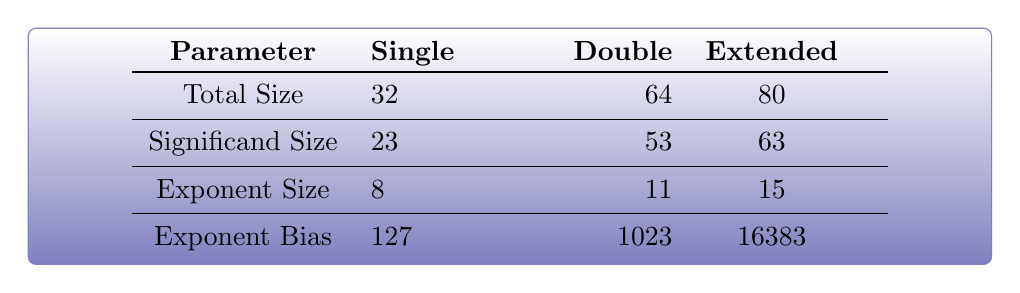
\begin{tikzpicture}[tab_style/.style={
	draw=blue!50!black!50,
	top color=white,
	bottom color=blue!50!black!50,
	rounded corners=1mm,
	text width=12cm,
	align=center
}]

\node[tab_style] {
\begin{tabularx}{.8\textwidth}{cXrccc}
\textbf{Parameter} & \textbf{Single} & \textbf{Double} & \textbf{Extended} \\
\toprule
Total Size &	32	&	64	&	80  &\\
\midrule
Significand Size & 23 & 53 & 63 &\\
\midrule
Exponent Size & 8 & 11 & 15 &\\
\midrule
Exponent Bias & 127 & 1023 & 16383 &\\

\end{tabularx}
};

\end{tikzpicture}
\end{document}